% Please make sure you insert your
% data according to the instructions in PoSauthmanual.pdf
\documentclass[a4paper,11pt]{article}
\usepackage{pos}
\usepackage{xspace}
\usepackage{subcaption}

\title{Euclid preparation: sensitivity to neutrino parameters}
%% \ShortTitle{Short Title for header}

\newcommand{\euclid}{\textit{Euclid}\xspace}
\newcommand{\planck}{\textit{Planck}\xspace}

\newcommand{\dneff}{\Delta N_\mathrm{eff}}
\newcommand{\summnu}{\sum m_\nu}

\newcommand{\threetimestwo}{3$\times$2\,pt}

\newcommand{\camb}{\texttt{CAMB}\xspace}
\newcommand{\class}{\texttt{CLASS}\xspace}
\newcommand{\montepython}{\texttt{MontePython}\xspace}
\newcommand{\cosmicfish}{\texttt{CosmicFish}\xspace}

\author[1,2]{ M.~Archidiacono}
\author[3]{ J.~Lesgourgues}
\author[3]{ S.~Casas}
\author*[3]{ S.~Pamuk}
\author[4]{ N.~Sch\"oneberg}
\author[5,6,7]{ Z.~Sakr}
\author[8,9,10]{ G.~Parimbelli}
\author[11]{ A.~Schneider}
\author[12,11]{ F.~Hervas~Peters}
\author[13,14,15]{ F.~Pace}
\author[3,16]{ V.~M.~Sabarish}
\author[17,18,19]{ M.~Costanzi}
\author[13,14,15]{ S.~Camera}
\author[20]{ C.~Carbone}
\author[21]{ S.~Clesse}
\author[22]{ N.~Frusciante}
\author[23,19]{ A.~Fumagalli}
\author[17,18,24,19]{ P.~Monaco}
\author[25]{ D.~Scott}
\author[19,18,10,24,26]{ M.~Viel}

\affiliation[1]{Dipartimento di Fisica "Aldo Pontremoli", Universit\`a degli Studi di Milano, Via Celoria 16, 20133 Milano, Italy}
\affiliation[2]{INFN-Sezione di Milano, Via Celoria 16, 20133 Milano, Italy}
\affiliation[3]{Institute for Theoretical Particle Physics and Cosmology (TTK), RWTH Aachen University, 52056 Aachen, Germany}
\affiliation[4]{Institut de Ci\`{e}ncies del Cosmos (ICCUB), Universitat de Barcelona (IEEC-UB), Mart\'{i} i Franqu\`{e}s 1, 08028 Barcelona, Spain}
\affiliation[5]{Institut f\"ur Theoretische Physik, University of Heidelberg, Philosophenweg 16, 69120 Heidelberg, Germany}
\affiliation[6]{Institut de Recherche en Astrophysique et Plan\'etologie (IRAP), Universit\'e de Toulouse, CNRS, UPS, CNES, 14 Av. Edouard Belin, 31400 Toulouse, France}
\affiliation[7]{Universit\'e St Joseph; Faculty of Sciences, Beirut, Lebanon}
\affiliation[8]{Institute of Space Sciences (ICE, CSIC), Campus UAB, Carrer de Can Magrans, s/n, 08193 Barcelona, Spain}
\affiliation[9]{Dipartimento di Fisica, Universit\`a degli studi di Genova, and INFN-Sezione di Genova, via Dodecaneso 33, 16146, Genova, Italy}
\affiliation[10]{SISSA, International School for Advanced Studies, Via Bonomea 265, 34136 Trieste TS, Italy}
\affiliation[11]{Department of Astrophysics, University of Zurich, Winterthurerstrasse 190, 8057 Zurich, Switzerland}
\affiliation[12]{AIM, CEA, CNRS, Universit\'{e} Paris-Saclay, Universit\'{e} de Paris, 91191 Gif-sur-Yvette, France}
\affiliation[13]{Dipartimento di Fisica, Universit\`a degli Studi di Torino, Via P. Giuria 1, 10125 Torino, Italy}
\affiliation[14]{INFN-Sezione di Torino, Via P. Giuria 1, 10125 Torino, Italy}
\affiliation[15]{INAF-Osservatorio Astrofisico di Torino, Via Osservatorio 20, 10025 Pino Torinese (TO), Italy}
\affiliation[16]{Hamburger Sternwarte, University of Hamburg, Gojenbergsweg 112, 21029 Hamburg, Germany}
\affiliation[17]{Dipartimento di Fisica - Sezione di Astronomia, Universit\`a di Trieste, Via Tiepolo 11, 34131 Trieste, Italy}
\affiliation[18]{INAF-Osservatorio Astronomico di Trieste, Via G. B. Tiepolo 11, 34143 Trieste, Italy}
\affiliation[19]{IFPU, Institute for Fundamental Physics of the Universe, via Beirut 2, 34151 Trieste, Italy}
\affiliation[20]{INAF-IASF Milano, Via Alfonso Corti 12, 20133 Milano, Italy}
\affiliation[21]{Universit\'e Libre de Bruxelles (ULB), Service de Physique Th\'eorique CP225, Boulevard du Triophe, 1050 Bruxelles, Belgium}
\affiliation[22]{Department of Physics "E. Pancini", University Federico II, Via Cinthia 6, 80126, Napoli, Italy}
\affiliation[23]{Ludwig-Maximilians-University, Schellingstrasse 4, 80799 Munich, Germany}
\affiliation[24]{INFN, Sezione di Trieste, Via Valerio 2, 34127 Trieste TS, Italy}
\affiliation[25]{Department of Physics and Astronomy, University of British Columbia, Vancouver, BC V6T 1Z1, Canada}
\affiliation[26]{ICSC - Centro Nazionale di Ricerca in High Performance Computing, Big Data e Quantum Computing, Via Magnanelli 2, Bologna, Italy}

\emailAdd{pamuk@ifca.unican.es}

\abstract{The European Space Agency has launched its newest mission in July 2023. The Euclid mission is planned to create one of the largest galaxy clustering and weak gravitational lensing survey to its date. The complimentary of a wide photometric redshift galaxy survey and spectroscopic survey will provide excellent sensitivity to the history of structure foramtion.\\
The following presents the newest forecast of \euclid done within the collaboration for the mission's main cosmological probes to see how well future data from \euclid will be able to constrain parameters from Neutrino physics. This forecast is focused on the summed mass of neutrino species $\summnu$, as well as the effective number of additional ultra relativistic species $\dneff$.\\
We show how the upcoming data could lead to unprecedented sensitivity in these parameters and could, together with data from future cosmic microwave background experiments, be able to have a detection of the neutrino mass scale.}

\FullConference{12th Neutrino Oscillation Workshop (NOW2024)\\
 2-8, September 2024\\
Otranto, Lecce, Italy\\}

%% \tableofcontents

\begin{document}
\maketitle


\section{Background}
The \euclid mission\cite{euclidcollaboration2024euclidiovervieweuclid} is planned to measure the location and shape of close to a billion galaxies over approximately one third of the sky. With a look back time of roughly ten billion years, \euclid will produce the largest galaxy catalogue to date. The cosmological information that can be obtained from this can be used to measure the cosmological neutrino mass, $\sum m_\nu$, as well as the effective number of additional ultra-relativistic relics, $\Delta N_\mathrm{eff}$.\\
The effect of these quantities on cosmological observables are described in \cite{ParticleDataGroup:2024cfk, Vagnozzi_2018, ISTF2020}. In the following section, we will briefly introduce these observables.

The observable that is mainly constraining the cosmological neutrino mass is the weak lensing (WL) probe.
The shapes of background (source) galaxies correlate with each other as they are get lensed by the same foreground (lens) galaxies. This correlation can be directly related to the correlation of the underlying matter field. Adding massive neutrinos suppresses this correlation in a scale dependent way, as it slows down the formation of structure for scales where the neutrinos are free-streaming i.e. where they are still to hot to cluster inside of gravitational wells.
Measuring the WL signal gives a unique method to directly measure the overall amplitude of the matter perturbations   

The next probe of interest is the Galaxy clustering (GC) probe, where we measure the spacial correlation of galaxies. In the standard cosmological model the matter perturbations all originate from primordial perturbations generated during inflation. At early times these perturbations generated pressure waves (acoustic waves) in the tightly coupled radiation matter fluid. These pressure waves are frozen when radiation and matter decoupled at recombination. This creates an excess in the measured correlation function at the size of these acoustic waves (BAO). The size of these waves depends on the expansion history of the universe. Adding additional massless relics through $\dneff$ or changing the fraction of matter that was still relativistic at recombination through $\summnu$ creates a measurable signal in the BAO.

Additionally to the BAO, the amplitude of the GC signal is also given by the underlying matter distribution. As galaxies form in over dense regions an over density in the galaxy distribution is related to the over density in the total matter. Contrary the the WL signal this relation is not a direct correspondence, rather the galaxy field is a bias tracer of the galaxy field. In the linear bias model this relation is modelled through a proportionality constant $b$ called the galaxy bias. Alone the GC probe could only be able to measure the amplitude of matter perturbations times this bias. \euclid will be able to construct the GC power spectrum using photometric redshifts, as well using spectroscopic ones. While the galaxies for which we have measured photometric redshifts will mainly be used after binning them in tomographic redshift bins, the spectroscopic redshift measurements will allow for the computation of the three-dimensional redshift space power spectrum. We denote these two probes as GCph and GCsp respectively.

The combination of the WL and GC probe can be used to break possible degeneracies and really measure the distribution of matter, making the measurement of $\summnu$ through GC probes possible. There is additional information in the cross correlation (XC) of these two probes. As the source galaxies get lensed by the foreground structure that the lensing galaxies trace, the XC becomes very natural. From these probes three probes---GCph, WL, and XC---we extract the two point statistics.

Additionally to these probes we additionally add information from redshift space distortions (RSD) and the cosmic microwave background (CMB) to further constrain neutrino parameters and break possible degeneracies.

\section{Methodology}

The forecast is done using Markov chain Monte Carlo (MCMC) methods to go beyond the standard Fisher information (FI) formalism. This is done, as we expect deviations from Gaussian posteriors for the neutrino parameters, as well as to add physical priors edges at a zero neutrino mass.

The validation of our forecast was done in 3 separate steps. In the first step we validated our Einstein--Boltzmann solver (EBS) by performing multiple FI forecasts where we have compared different EBSs. For this forecast we used the \cosmicfish code that was validated before within the efforts of the Euclid consortium\cite{ISTF2020}. The two most common EBSs are \camb\cite{2011ascl.soft02026L} and \class\cite{Diego_Blas_2011}. Even though they have been validated in the past, we did the validation again. This is because \euclid will have unprecedented precision on the measurement of the matter power spectrum and thus we have to be sure that our results do not depend on the particular code used. Furthermore the \euclid observables will need us to have a good handle on the non-linear corrections to the power spectrum. We performed a thorough analysis of multiple recipes for these non-linear corrections and compared them to N-body simulations. In the presence of massive neutrinos, the best comparison was achieved with the \texttt{HMCode2020} recipe \cite{Mead_2021}. Like this, the \texttt{HMCode2020} recipes within \class and \camb were validated for the first time.

We then formulated a likelihood for \montepython\cite{Audren:2012wb} as an extension to the existing likelihood formulated in \cite{casas2023euclidvalidationmontepythonforecasting}. To perform a robust forecast on the neutrino mass we used particular care to correctly model the measured signal. The scale-dependent suppression of growth due to neutrinos makes the galaxy bias a scale dependent quantity. This scale dependence has to be properly handled as it can bias the measured value and sensitivity for $\summnu$ \cite{Vagnozzi_2018}. As neutrinos did not cluster inside of halos, the RSD is driven by cold dark matter and baryonic matter only\cite{Villaescusa_Navarro_2018}. For this reason, the measured signal has to be additionally modified to describe this defect. In the second step, We validated our likelihood by performing a FI forecast with it. We compare the results to the ones of the first step.

Finally, we ran an MCMC using our \montepython likelihood to check for the validity of our FI forecast. Any deviations between MCMC and FI could be explained from non-Gaussianities of the posterior as well as from prior effects. With this we were sure that our previous validation was also valid for an MCMC forecast.

\section{Results}

The final forecast was performed using \montepython. We decided to vary different sets of cosmological parameters for the analysis to study how much the constraints degrade by opening up the parameter space. The baseline model consists of  five $\varLambda$CDM parameters as well as $\summnu$ i.e $\{h, \Omega_\mathrm{m}, \Omega_\mathrm{b}, \sigma_8, n_\mathrm{s}, \summnu\}$. We also studied what happens when opening up the number of additional massless relics $\{\dneff\}$, and/or the Chevallier--Polarski--Linder parameters for the equation of state of dark energy $\{w_0,w_a\}$. Additionally when adding additional information from CMB experiments we vary the optical depth of reionisation $\tau$. We assume flat cosmology and three massive neutrinos with degenerate masses. It was shown that the latter choice is appropriate as individual mass splittings are not resolvable with cosmological data\cite{Lesgourgues:2013sjj}.

We performed these forecasts for different combinations of the \euclid main probes as well as adding additional information from CMB experiments. For the survey specifications of \euclid we stick to the pessimistic settings outlined in \cite{ISTF2020}. We consider two cases for the CMB experiments: We either use a mock likelihood for \planck or for a more futuristic setup of CMB-S4 + LiteBird.

For the combination of the main \euclid probes we find in the baseline model a sensitivity to the cosmological neutrino mass of $\sigma\left(\summnu\right) = 56\,\mathrm{meV}$. This degrades to an 95\% confidence level (CL) of $\summnu<220\,\mathrm{meV}$ when opening up $\dneff$. In this case the posterior is compatible with a 0 mass at the 1-$\sigma$ level and thus could bias the reported uncertainty. For $\dneff$ we find an upper bound of $\dneff<0.746$ at a 95\% CL. Additionally opening up the dark energy equation of state does not measurably degrade the sensitivity to $\summnu$ while the 95\% CL of $\dneff$ degrades to $\dneff<0.935$.  

Adding CMB to this tightens the constraints in the full 10 parameter model to $\sigma\left(\summnu\right) = 40\,\mathrm{meV}$ or $\sigma\left(\summnu\right) = 31\,\mathrm{meV}$ for \planck or CMB-S4+LiteBird respectively. The constraints on $\dneff$ are dominated by CMB probes but the main degeneracy of $\dneff$ with the local expansion speed of the universe $h$ is broken though the \euclid data. Like this the combination of \euclid and CMB data could provide unprecedented sensitivity to $\dneff$ with a forecast sensitivity of $\dneff<0.149$ or $\dneff<0.069$ for \euclid + \planck or \euclid + CMB-S4 + LiteBird respectively. 

The forecast sensitivities are put in a physical context in figure \ref{fig:results}.

\begin{figure}[!htbp]
    \centering
    \begin{subfigure}{0.49\textwidth}
        \centering
        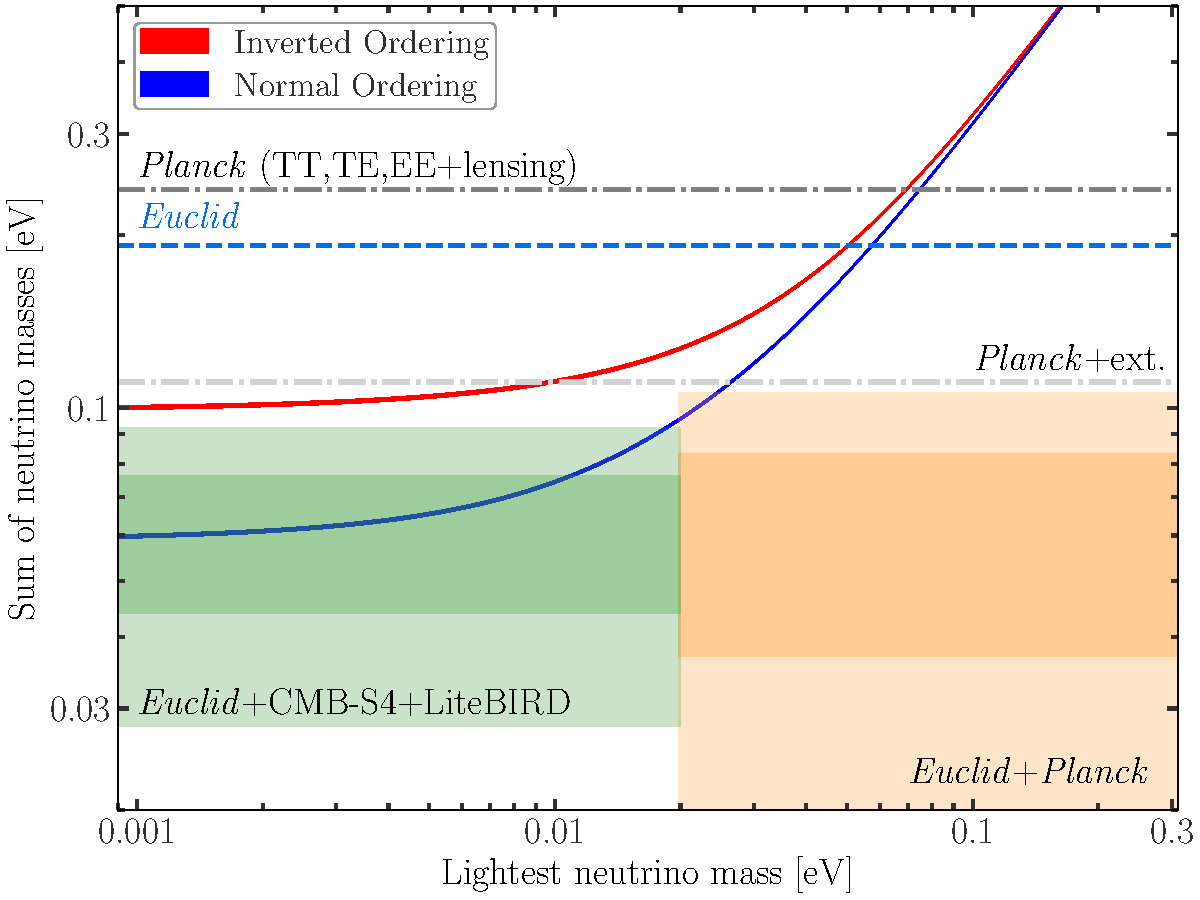
\includegraphics[width=\linewidth]{figure_hierarchy-1.pdf}
    \end{subfigure}
    \hfill
    \begin{subfigure}{0.49\textwidth}
        \centering
        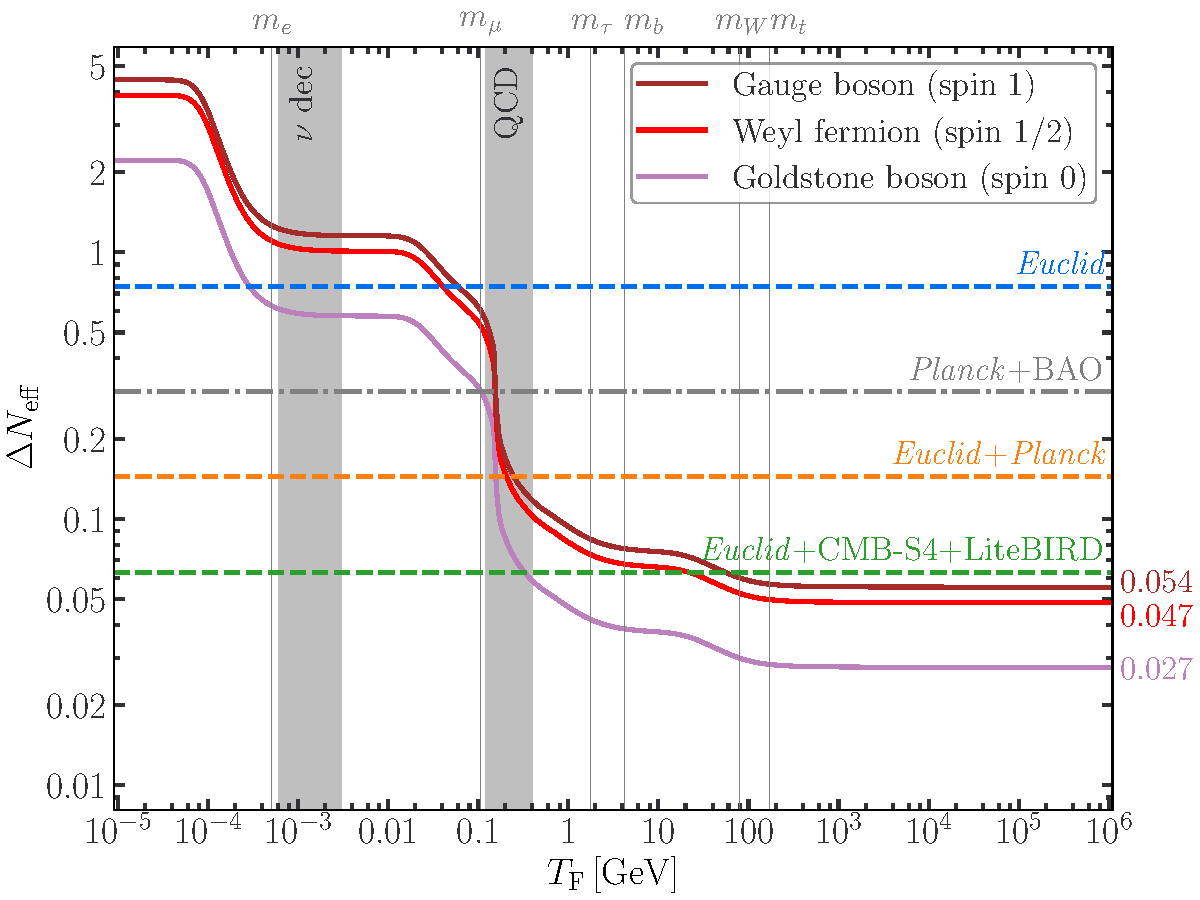
\includegraphics[width=\linewidth]{figure_Neff-1.pdf}
    \end{subfigure}
    \caption{\textit{left}, forecast sensitivity for the $\summnu$ for different combinations of \euclid with or without external CMB data. We compare the sensitivities to current measurements of \planck or \planck + additional data from supernovae, BAO measurements and current large scale structure measurements. The dashed lines represent the 95\% CL. The strike-through lines represent the sum of the neutrino masses from oscillation experiments depending on the ordering and the lowest neutrino mass. We show how for the minimal mass scenario \euclid + CMB could be able to differentiate normal or inverted ordering.;\\
    \textit{right}, Similar to the left plot but for the sensitivity for $\dneff$. The strike-through lines represent contritubtions to $\dneff$ from different types of particles and different decoupling temperatures. We show how with future CMB experiments \euclid will be able to exclude models with additional relics decoupling even before the QCD phase transition.
    }
    \label{fig:results}
\end{figure}

\bibliographystyle{JHEP}
\bibliography{my-bib-database}

\end{document}
